\documentclass[]{article}
\usepackage{lmodern}
\usepackage{amssymb,amsmath}
\usepackage{ifxetex,ifluatex}
\usepackage{fixltx2e} % provides \textsubscript
\ifnum 0\ifxetex 1\fi\ifluatex 1\fi=0 % if pdftex
  \usepackage[T1]{fontenc}
  \usepackage[utf8]{inputenc}
\else % if luatex or xelatex
  \ifxetex
    \usepackage{mathspec}
    \usepackage{xltxtra,xunicode}
  \else
    \usepackage{fontspec}
  \fi
  \defaultfontfeatures{Mapping=tex-text,Scale=MatchLowercase}
  \newcommand{\euro}{€}
\fi
% use upquote if available, for straight quotes in verbatim environments
\IfFileExists{upquote.sty}{\usepackage{upquote}}{}
% use microtype if available
\IfFileExists{microtype.sty}{%
\usepackage{microtype}
\UseMicrotypeSet[protrusion]{basicmath} % disable protrusion for tt fonts
}{}
\usepackage[margin=1in]{geometry}
\usepackage{graphicx}
\makeatletter
\def\maxwidth{\ifdim\Gin@nat@width>\linewidth\linewidth\else\Gin@nat@width\fi}
\def\maxheight{\ifdim\Gin@nat@height>\textheight\textheight\else\Gin@nat@height\fi}
\makeatother
% Scale images if necessary, so that they will not overflow the page
% margins by default, and it is still possible to overwrite the defaults
% using explicit options in \includegraphics[width, height, ...]{}
\setkeys{Gin}{width=\maxwidth,height=\maxheight,keepaspectratio}
\ifxetex
  \usepackage[setpagesize=false, % page size defined by xetex
              unicode=false, % unicode breaks when used with xetex
              xetex]{hyperref}
\else
  \usepackage[unicode=true]{hyperref}
\fi
\hypersetup{breaklinks=true,
            bookmarks=true,
            pdfauthor={Zhenyuan Shen (NetID: zshen52)},
            pdftitle={ME/ECE/EMA/CS 759 High Performance Computing for Engineering Applications Assignment 8},
            colorlinks=true,
            citecolor=blue,
            urlcolor=blue,
            linkcolor=magenta,
            pdfborder={0 0 0}}
\urlstyle{same}  % don't use monospace font for urls
\setlength{\parindent}{0pt}
\setlength{\parskip}{6pt plus 2pt minus 1pt}
\setlength{\emergencystretch}{3em}  % prevent overfull lines
\setcounter{secnumdepth}{0}

%%% Use protect on footnotes to avoid problems with footnotes in titles
\let\rmarkdownfootnote\footnote%
\def\footnote{\protect\rmarkdownfootnote}

%%% Change title format to be more compact
\usepackage{titling}

% Create subtitle command for use in maketitle
\newcommand{\subtitle}[1]{
  \posttitle{
    \begin{center}\large#1\end{center}
    }
}

\setlength{\droptitle}{-2em}
  \title{ME/ECE/EMA/CS 759 High Performance Computing for Engineering
Applications Assignment 8}
  \pretitle{\vspace{\droptitle}\centering\huge}
  \posttitle{\par}
  \author{Zhenyuan Shen (NetID: zshen52)}
  \preauthor{\centering\large\emph}
  \postauthor{\par}
  \predate{\centering\large\emph}
  \postdate{\par}
  \date{November 07, 2015}



\begin{document}

\maketitle


\begin{enumerate}
\def\labelenumi{(\Alph{enumi})}
\item
  In each iteration, this tiled-solution handles BLOCK\_SIZE consecutive
  elements of the array and pass the sum of the subarray to the next
  iteration to push the next iteration forward, which will be able to
  deal with more than 2048 elements.
\item
  Implement a work scan algorithm to get O(nlog(n)) performance with
  Hillis and Steele's.
\item
  This solution can handle non-power of 2 array sizes by discarding the
  invalid out-of-bound values.
\item
  This solution has shared memory bank conflicts since the strides are
  the power of 2.
\end{enumerate}

\begin{quote}
Usage: ./scan {[}arguments{]}
\end{quote}

\begin{quote}
Profiling: sbatch scriptTiming.sh
\end{quote}

Results

Time cost:

Processing 16777216 elements\ldots{}

Host CPU Processing time: 78.476257 (ms)

GPU inclusive time: 169.659515 (ms)

Speedup: 0.462551X

Test PASSED

Profiling:

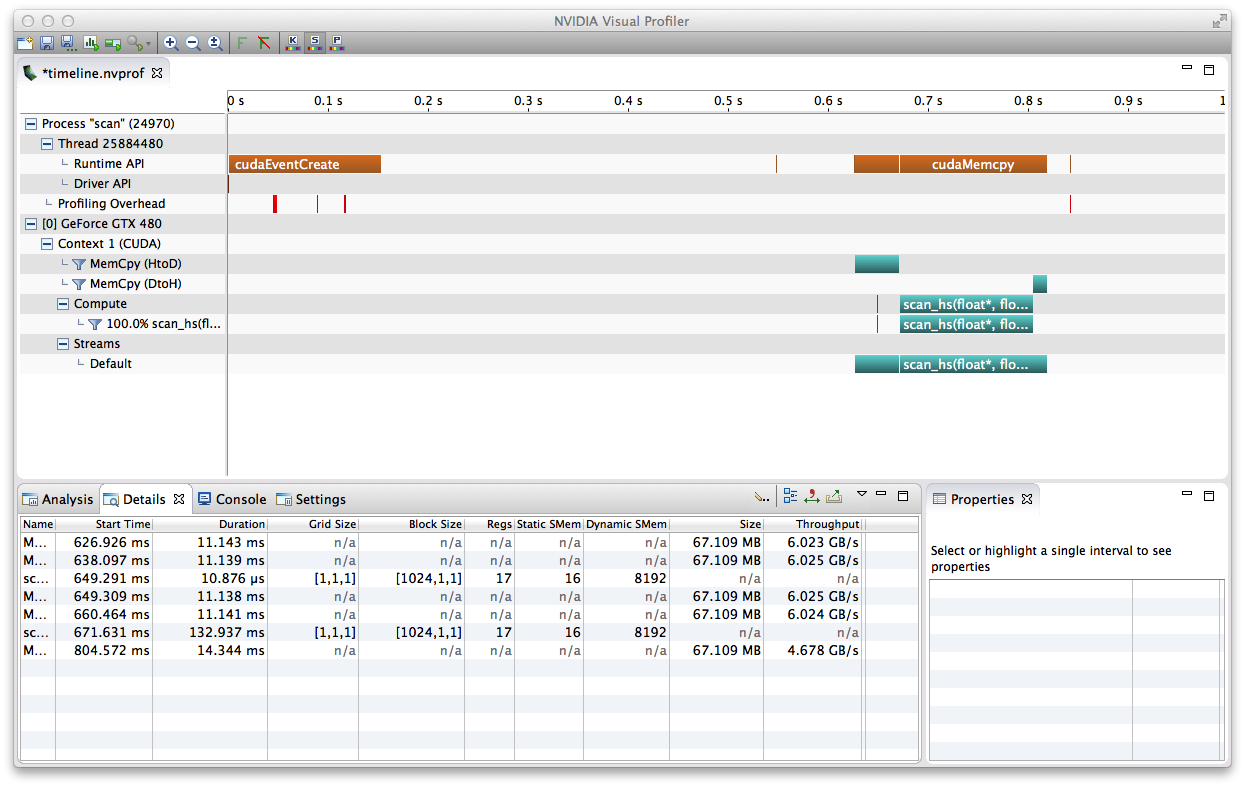
\includegraphics{./hw08.png}

From the profiling above,

Memcpy DtoH: duration = 14.344ms , throughput = 4.678GB/s

Memcpy HtoD: avg. duration = 11.141ms , avg. throughput = 6.024GB/s

GPU executing: duration = 132.937ms

\end{document}
